\chapter{System Design}\label{ch:appendix_design}
This appendix show the overall design of the system in UML layer, class and
sequence diagrams.

\section{VN implementation high-level design}\label{sec:layered_design}
TODO:

\section{Component and Service discovery process}\label{sec:discovery_process}
The following sequence diagrams show the basic component and service discovery
process for a local subnet using UDP/IP for inter-process communication
described in SPA Local Subnet Adaptation Draft \cite{spa:local-subnet}.

Figure
\ref{fig:appendix_vn_discovery_overview} starts with the high-level view of a
complete SPA network. Figure
\ref{fig:appendix_vn_local_subnet_network_discovery} continues with the
specifics of a SPA Local Subnet. Figure
\ref{fig:appendix_vn_address_block_assignment} shows the specifics on how a SPA
Subnet Manager aquires an address block from the CAS and after that the SPA
Subnet Manager assigns a logical address to each component it is aware of in
figure \ref{fig:appendix_vn_local_subnet_address_assignment}. The last step is the
component capabilities discovery process where the LS collects
information about all known components on the network, this is shown in figure
\ref{fig:appendix_vn_component_capabilities_discovery}.

\begin{figure}[h]
    \centering
    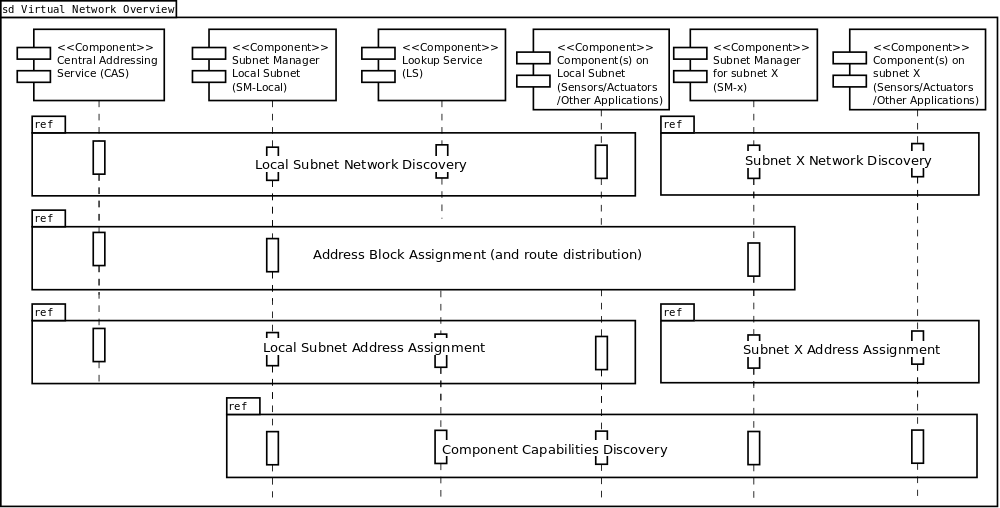
\includegraphics[width=\textwidth]{figures/vn_discovery_overview}
    \caption{Overview of the discovery process for a SPA network.}
    \label{fig:appendix_vn_discovery_overview}
\end{figure}

\begin{figure}[h]
    \centering
    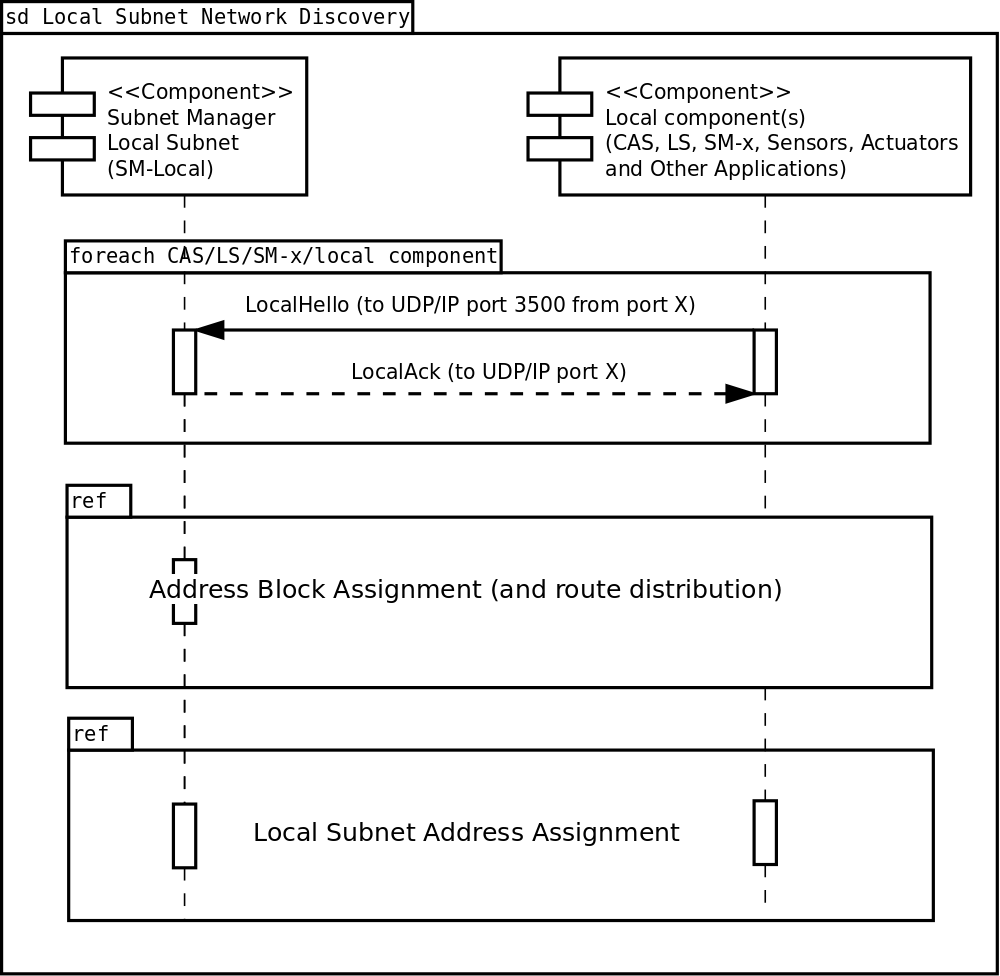
\includegraphics[width=\textwidth]{figures/vn_local_subnet_network_discovery}
    \caption{The basic discovery process for a SPA Local Subnet Discovery.}
    \label{fig:appendix_vn_local_subnet_network_discovery}
\end{figure}

\begin{figure}[h]
    \centering
    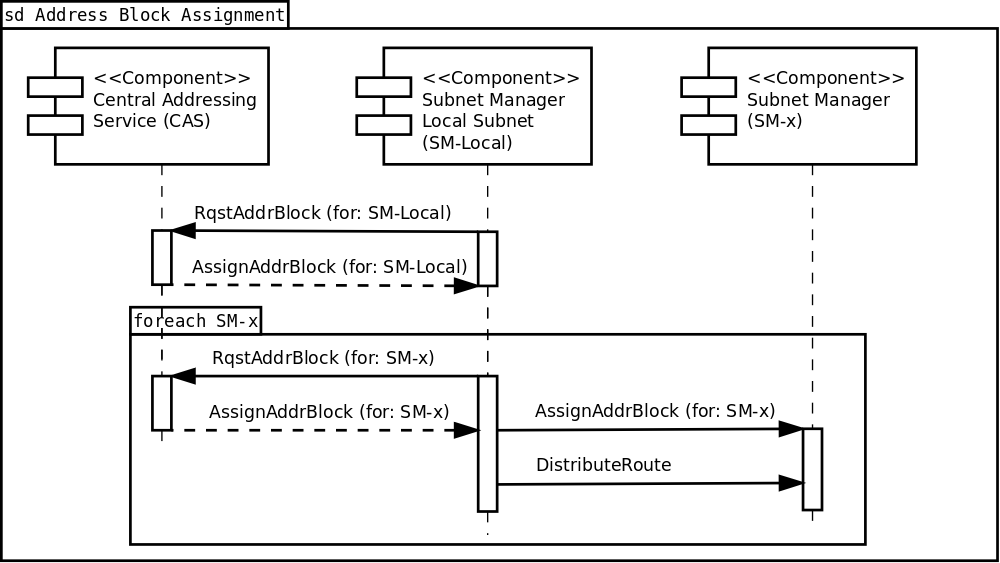
\includegraphics[width=\textwidth]{figures/vn_address_block_assignment}
    \caption{How the local subnet manager aquires address block from the CAS
    for its own subnet and for other connected subnet managers.}
    \label{fig:appendix_vn_address_block_assignment}
\end{figure}

\begin{figure}[h]
    \centering
    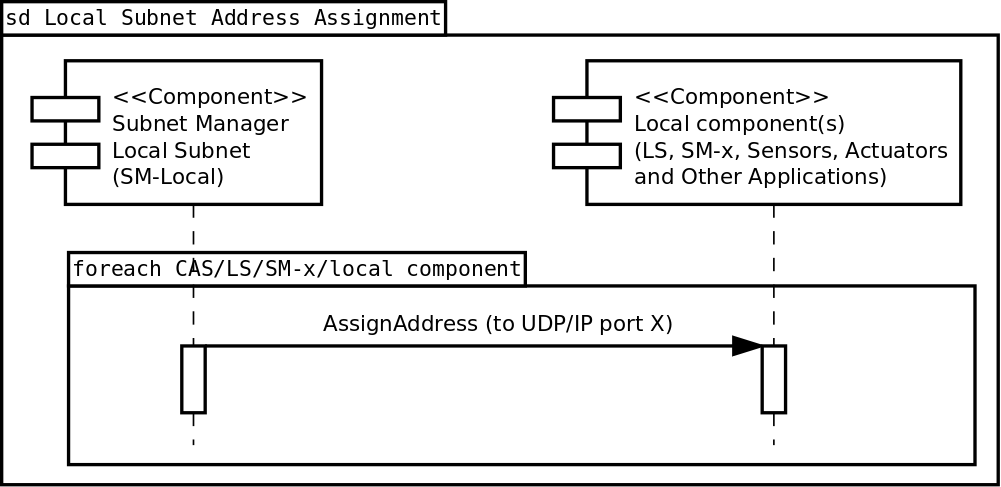
\includegraphics[width=\textwidth]{figures/vn_local_subnet_address_assignment}
    \caption{After the SM-L has received Address Block it starts to assign
    logical addresses to local components it's aware of.}
    \label{fig:appendix_vn_local_subnet_address_assignment}
\end{figure}

\begin{figure}[h]
    \centering
    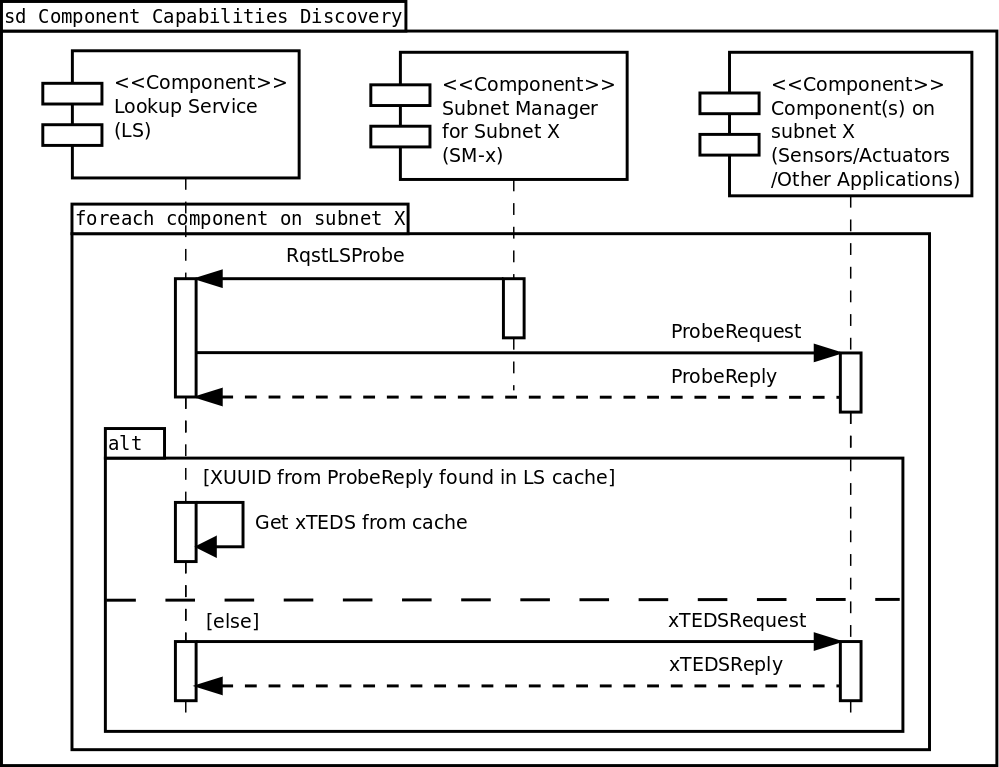
\includegraphics[width=\textwidth]{figures/vn_component_capabilities_discovery}
    \caption{The last step in the discovery process is to discovery which
    components have which services, capabilities that is.}
    \label{fig:appendix_vn_component_capabilities_discovery}
\end{figure}
